\section{Overview}
\label{sec:overview}

This section provides some background on union types, and some common approaches
to eliminate union types. Then it describes the Ceylon approach to Union types.
Finally, it presents the key ideas and challenges in our work and \name.

\subsection{Tagged Union Types}

% Brief intro to union types and one or 2 simple examples that show that we
% can automatically lift values into union type without the need of some
% tag/constructor. Something like:

We start with a brief introduction to union types. An expression has a union
type $[[A\/B]]$, if it can be considered to have either type $[[A]]$ \textit{or}
type $[[B]]$. Many systems model \textit{tagged union types} (also called
\textit{sum types} or \textit{variants types}), where explicit \textit{tags}
are used to construct terms with union types. Languages with algebraic datatypes~\cite{hope}
or (polymorphic) variants~\cite{garrigue98} support tagged union types.
In their basic form, there are two introduction forms:
$\mathsf{inj_1} :: [[A -> A \/ B]]$ turn the type of an expression of type
$[[A]]$ into type $[[A \/ B]]$; and $\mathsf{inj_2} :: [[B -> A \/ B]]$
turns the type of an expressions of type $[[B]]$ into type $[[A \/ B]]$
For example, we can have:

\begin{lstlisting}
inj1 "foo": String | Int
inj2 1 : String | Int
\end{lstlisting}

\noindent Note that in the code above we write union types as
\lstinline{String | Int} (instead of $[[String \/ Int]]$),
since this is a common notation in many programming languages,
including Ceylon.
Using tagged union types, we can implement a safe integer
division function, as:

\begin{lstlisting}
function safediv (x : Int) (y : Int) : String | Int =
  if (y == 0) then inj1 "Divided by zero" else inj2 (x / y)
\end{lstlisting}

\noindent Here the intention is to have a safe (integer) division operation that detects
division by zero errors, and requires clients of this function to handle
such errors. The return type \lstinline{String | Int} denotes that the function
can either return an error message (a string), or an integer, when division
is performed without errors.

\paragraph{Eliminating tagged union types.}
Tagged union types are eliminated by some form of case analysis.
For consistency with the rest of the paper, we use a syntactic form with
\lstinline{switch} expressions for such case analysis. For example,
the following program \lstinline{tostring} has different behaviors depending on the
tag of \lstinline{x}, where \lstinline{show} takes an \lstinline{Int} and
returns back its string representation.

\begin{lstlisting}
function tostring (x: String | Int) : String = switch (x)
                                                 inj1 str -> str
                                                 inj2 num -> show num
\end{lstlisting}

\noindent Combining union type construction in \lstinline{safediv} and its elimination in
\lstinline{tostring}, we can easily implement an interface which returns the
result of safe division as one \lstinline{String}.

\begin{lstlisting}
> tostring (safediv 42 2)
"21"
> tostring (safe 42 0)
"Divided by zero"
\end{lstlisting}


\subsection{Type-directed Elimination of Union Types}\label{subsec:elimination}

% Motivate the need for having a construct that can eliminate union types,
% perhaps trying to use an example where the String above would be a kind
% of exception, and the Int would be regular computation. Alternatively
% find an existing example from the literature.

% Discussing existing approaches for eliminating union types;
% point out that elimination constructs based on types (our focus) vs
% elimination constructs based on tags (which are used in algebraic
% datatypes or polymorphic variants (like in OCaml)).
% The focus should be on type-based approaches.

% Try to identify some limitations/problems. For instance how to deal
% with ambiguity (just use order? restrict the construct somehow ...).


While tags are useful to make it explicit which type a value belongs to, they
also add clutter in the programs, and usually require extra space to store the
tags. On the other hand, in systems with subtyping for union types
\cite{dunfield2014elaborating,pierce1991programming,muehlboeck2018empowering},
explicit tags are replaced by implicit coercions represented by the two
subtyping rules $[[A <: A \/ B]]$ and $[[B <: A \/ B]]$. We call such types
\textit{untagged union types}, or simply \textit{union types}. In those systems,
a term of type $[[A]]$ or $[[B]]$ can be directly used as if it had type $[[A \/
B]]$, and thus we can model safe division as

\begin{lstlisting}
function safediv2 (x : Int) (y : Int) : String | Int =
  if (y == 0) then "Divided by zero" else (x / y)
\end{lstlisting}

\noindent However, now elimination of union types cannot rely on tags anymore, and
different systems implement elimination differently. We review some of the
existing approaches next.

\paragraph{Single branch elimination.}

A possible approach is to use an elimination of an expression with a union type
$[[A \/ B]]$ that supports only one branch. The branch needs to have the same
type when the expression has type $[[A]]$, or type $[[B]]$. This approach is
adopted, for example by \citet{pierce1991programming},
\citet{barbanera1995intersection}, and more recently,
\citet{dunfield2014elaborating}. For consistency with the presentation of this paper,
we adapt their syntax
using our switch notation in the examples, while preserving their semantics. For
example, in \lstinline{tostring2}, the expression \lstinline{show y} must return
\lstinline{String} when \lstinline{y : String}, and when \lstinline{y : Int},
which means that \lstinline{show} must be overloaded. In
\citet{pierce1991programming,dunfield2014elaborating,barbanera1995intersection},
this can be implemented by requiring \lstinline{show} to have an
\textit{intersection type} such as $[[(String -> String) /\ (Int -> String)]]$.
Then we can just write:

\begin{lstlisting}
function tostring2 (x: String | Int) : String = switch (x)
                                                  y -> show y
\end{lstlisting}

\noindent This implementation is concise, but it is also restrictive as it can no longer
support multiple branches according to the different representations of
\lstinline{x}. Furthermore it relies on the language also supporting overloaded
functions. Without overloaded functions the construct would not be very useful.
%\bruno{Perhaps, somewhere in this section we need to comment on the non-deterministic semantics.
%  Maybe we can do that here and point out, for instance, that Dunfield's approach has a
%  non-deterministic semantics (since it actually allows, for instance two overloaded
%  implementations of show with integer arguments)}

\paragraph{Type-directed elimination.}

On the other hand, some
systems~\cite{castagna:settheoretic} support
\textit{type-directed} elimination of union types. For instance,
\lstinline{tostring3} has different behaviors depending on the \textit{type} of
\lstinline{x}.

\begin{lstlisting}
function tostring3 (x: String | Int) : String = switch (x)
                                                  (y : String) -> y
                                                  (y : Int) -> show y
\end{lstlisting}

\noindent Note that here \lstinline{show} does not need to be overloaded,
as the type-directed elimination
\textit{turns} the variable \lstinline{x} of type \lstinline{String | Int} into
the variable \lstinline{y} of type \lstinline{Int}.

However, compared to tag-directed elimination, extra care must to taken with
type-directed elimination. In particular, while we can easily distinguish tags,
in type-directed elimination, ambiguity may arise when types in a union type
overlap. For example, consider the type \lstinline{Person | Student}, where we
assume \lstinline{Student} is a subtype of \lstinline{Person}. With tag-directed
elimination, we can write the following function:

\begin{lstlisting}
function isstudent (x: Person | Student) : Bool = switch (x)
                                                     inj1 person -> False
                                                     inj2 student -> True
\end{lstlisting}

\noindent But if we transform this function straightforwardly to type-directed
elimination, we will get:

\begin{lstlisting}
function isstudent2 (x: Person | Student) : Bool = switch (x)
                                                     (y : Person)  -> False
                                                     (y : Student) -> True
\end{lstlisting}

\noindent Now it is unclear what would happen if we apply \lstinline{isstudent2}
to a term of type \lstinline{Student}, as its type matches both branches. In
some calculi~\citep{dunfield2014elaborating}, the choice is not determined in
the semantics, in the sense that either branch can be chosen. This leads to a
non-deterministic semantics. In some other languages or
calculi~\citep{castagna:settheoretic}, branches are inspected from top to
bottom, and the first one that matches the type gets chosen. However, in those
systems, as \lstinline{Person} is a supertype of \lstinline{Student}, the first
branch subsumes the second one and will always get chosen, and so the second
branch will never get evaluated! This could be unintentional, and similar
programs being accepted could lead to subtle bugs. Even if a warning could be
given to alert programmers that a case can never be executed, there could be
other situations where two cases overlap, but neither case subsumes the other.
For instance we could have \lstinline{Student} and \lstinline{Worker} as
subtypes of \lstinline{Person}. For a person that is both a student and a
worker, a switch statement that discriminates between workers and students could
potentially choose either branch. However for persons that are only students or
only workers, only one branch can be chosen.

\paragraph{Best-match and overloading.}
Some languages support an alternative to typed-based union elimination via method
overloading. Such form is used in, for example, Java \cite{javadoc}. In Java, we
can encode \lstinline{isstudent3} as a function, which has different
behaviors when the type of the argument differs.

\begin{lstlisting}
boolean isstudent3 (Person x) { return False; }
boolean isstudent3 (Student x) { return True; }
\end{lstlisting}

\noindent Java resolves overloading by finding in all method implementations the one with
the \textit{best} type signature that describes the argument. If we
apply \lstinline{isstudent3} to a term of type \lstinline{Student}, the second
implementation is chosen, as \lstinline{Student} is the best type describing the
argument. As we can see, such best-match strategy gets rid of the
order-sensitive problem, as Java always try to find the best-match one despite
the order of the methods. In other words, in Java the order of methods does not matter:
in this case,
we have the method for \lstinline{Person} before the one for \lstinline{Student}, but Java still finds
the one for \lstinline{Student}.

However, the best-match strategy can also be confusing, especially when the
system features implicit upcasting (e.g., by subtyping). If programmers
are not very familiar with how overloading resolution works, they may assume
that the wrong implementation is called in their code. For instance, in Java
we may write:

\begin{lstlisting}
Person p = new Student();
p.isstudent3();
\end{lstlisting}

\noindent In this case Java will pick the \lstinline{isstudent3} method with the
argument \lstinline{Person}, since Java overloading uses the \emph{static type}
(\lstinline{p} has the static type \lstinline{Person})
to resolve overloading. But some programmers may assume that the implementation
of the method for \lstinline{Student} would be chosen instead, since the person
is indeed a student in this case. This can be confusing and lead to subtle bugs.

Moreover there are other tricky situations
that arize when employing a best-match strategy. For example, suppose
that the type \lstinline{Pegasus} is a subtype of both type \lstinline{Bird} and type
\lstinline{Horse}. If a method \lstinline{isbird} is overloaded for
\lstinline{Bird} and \lstinline{Horse}, then which method implementation should
we choose when we apply \lstinline{isbird} to a term of type
\lstinline{Pegasus}, the one for \lstinline{Bird}, or the one for
\lstinline{Horse}? In such case, we have an ambiguity. Things get worse
when the type system includes more advanced type system features, such as generics,
intersections and union types,
or type-inference.


%the semantics is non-deterministic again, and
%the behavior of the program depends on the particular implementation of the
%compiler.%\bruno{Should we use Worker/Student/Person here to be}


\subsection{Eliminating Union Types in Ceylon}

The Ceylon language~\cite{king2013ceylon} supports type-directed union elimination by a
switch expression with multiple branches. The following program is an example
with union types using Ceylon's syntax:

\begin{lstlisting}
void print(String|Integer|Float x) {
	switch (x)
	case (is String) { print("String: ``x``"); }
	case (is Integer|Float) { print("Number: ``x``"); }
}
\end{lstlisting}
%

For the switch expression, Ceylon enforces static type checking with two
guarantees: \textit{exhaustiveness}, and \textit{disjointness}. First, Ceylon
ensures that all cases in a switch expression are \textit{exhaustive}. In the above
example, \lstinline{x} can be either a string, an integer or a floating point
number. The types used in the cases do not have to exactly match with the types
of \lstinline{x}. Nevertheless, the combination of all cases must be able to
handle all possibilities. If the last case only dealt with
\lstinline{Integer} (instead of \lstinline{Integer|Float}), then the program
would be statically rejected, since no case would deal with a floating point
number.

Second, Ceylon enforces that all cases in a switch expression are
\textit{disjoint}. That is, unlike the approaches described in
Section~\ref{subsec:elimination}, in Ceylon, it is impossible to have two
branches that match with the input at the same time. For instance, if the first
case used the type \lstinline{String | Float} instead of \lstinline{String}, the
program would be rejected statically with a type error. Indeed, if the program
were to be accepted, then the call \lstinline{print(3.0)} would be ambiguous,
since there are two branches that could deal with the floating point number. Note that, since
the cases in a switch cannot overlap, their order is irrelevant to the program's
behavior and its evaluation result.

\paragraph{Union types as an alternative to overloading}
One motivation of such type-directed union elimination in Ceylon is to
model a form of function overloading.
The following example, which is adapted from TypeScript's documentation\footnote{\url{https://www.typescriptlang.org/docs/handbook/unions-and-intersections.html}},
demonstrates how to define an ``overloaded'' function \lstinline{padLeft},
which adds some padding to a string. The idea is that there can be two versions
of \lstinline{padLeft}: one where the second argument is a string; and
the other where the second argument is an integer:

\begin{lstlisting}
String space(Integer n){
  if (n==0) { return ""; }
  else { return " "+space(n-1); }
}
String padLeft(String v, String|Integer x) {
	switch (x)
	case (is String) { return x+v; }
	case (is Integer) { return space(x)+v; }
}
print( padLeft("?", 5) ); // "     ?"
print( padLeft("World", "Hello ") ); // "Hello World"
\end{lstlisting}
%

\noindent In two cases of the switch construct, there are two different implementations
of the \lstinline{padLeft} function: one that appends a string to the left of \lstinline{v},
and the other that calls function \lstinline{space} to generate a string with \lstinline{x} spaces,
and then append that to \lstinline{v}.
Although statically \lstinline{x} has type \lstinline{String|Integer}, as a concrete value
it can only be a string or an integer.
As such, when values with such types are passed to the function,
the corresponding branch is chosen and executed.

\paragraph{Other applications of union types}
\begin{wrapfigure}{R}{0.35\textwidth}
\tikzset{
  state/.style={
    rectangle,
    rounded corners,
    minimum height=2em,
    inner sep=2pt,
    text centered,
    align=center
  },
}
\begin{center}
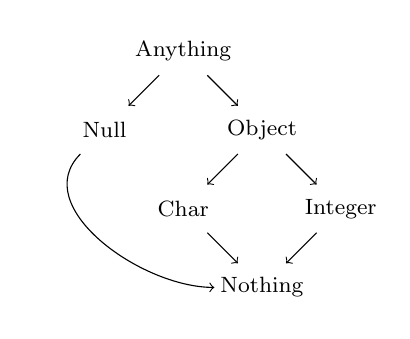
\begin{tikzpicture}[->]
  \footnotesize
  \node[state, anchor=center] (a) at (0, 0) {Null};
  \node[state, anchor=center] (b) at (2, 0) {Object};
  \node[state, anchor=center] (c) at (1, 1) {Anything};
  \node[state, anchor=center] (d) at (1, -1) {Char};
  \node[state, anchor=center] (e) at (3, -1) {Integer};
  \node[state, anchor=center] (f) at (2, -2) {Nothing};
  \draw (c) -- (a);
  \draw (c) -- (b);
  \draw (b) -- (d);
  \draw (b) -- (e);
  \draw (e) -- (f);
  \draw (d) -- (f);
  \draw (a) to[out=225,in=180] (f);
\end{tikzpicture}
\end{center}
\end{wrapfigure}
Besides being used for overloading, union types can be used for other purposes too.
An interesting application of union types in Ceylon is to
encode \textit{nullable types} (or \textit{optional types}) in a type-safe way.
A similar approach to nullable types has also been recently proposed for
Scala~\citep{nieto20nulls}. In those languages, the type \lstinline{Null} is
inhabited by the \lstinline{null} value. The user can then write \lstinline{A?},
which stands for \lstinline{A|Null}, for a term of type \lstinline{A} to be
nullable. If we eliminate a value of type \lstinline{A|Null}, there has to be a
branch to handle the null value. Note that \lstinline{Null} differs from
\lstinline{Nothing} (the bottom type in Ceylon), in the sense that
\lstinline{Null} is inhabited while \lstinline{Nothing} is not. To illustrate
the subtle difference, the diagram on the right presents part of the subtyping
lattice in Ceylon. \lstinline{Anything}, the top type in Ceylon, is an
enumerated class. \lstinline{Anything} is also a supertype of
\lstinline{Object}, which is the root of primitive types, function types, all
interfaces and any user-defined class. Notably, \lstinline{Null} is disjoint to
\lstinline{Object}, and therefore, to all these types.

Moreover, union types can also be used for error handling.
We can easily encode the \lstinline{safediv} function in Section~\ref{subsec:elimination}
in Ceylon:
%
\begin{lstlisting}
String | Integer safediv3 (Integer x, Integer y){
  if (y==0) { return "Divided by zero"; }
  else { return (x/y); }
}
\end{lstlisting}
%
The return value can be a string or an integer.
No tag is needed for any of them to be a \lstinline{String|Integer},
since union types can be implicitly introduced.
For the declared return type of the function, as long as it is
a supertype of all possible return values, it is valid
in Ceylon.





%Similarly, one can use enumerated types to denote various special cases, or easily
%add another type to the argument type of an existing function when considering
%more possible inputs, to improve the program's robustness.
%Next, we will see how Ceylon's static type checking helps programmers.

\begin{comment}
\paragraph{Exhaustiveness}

Ceylon checks the exhaustiveness of a switch by comparing the union of all
cases and the switched term's type.
For the switch to be accepted, the former must be a supertype of the later.
%Recall that adding more components to a union type make it a supertype of the
%initial type, like \lstinline{Integer|Float} to \lstinline{Integer}.
That is to say a switch construct must have enough cases to handle all
possible runtime types of the term.
%
For example, here we define \lstinline{Node} by enumerating its subtypes.
It can be viewed as the union of \lstinline{Leaf} and \lstinline{Branch}.
Then in the function \lstinline{printTree} that takes a \lstinline{Node},
both cases are taken into consideration.
%
\begin{comment}
------------- THE OTHER EXAMPLE -----------------
Adding more subtype in it causes error in exhaustiveness checking in switch.
\begin{lstlisting}
interface Resource of File | Directory | Link { }
interface File satisfies Resource {}
interface Directory satisfies Resource {}
interface Link satisfies Resource {}

void printType(Resource resource){
	switch (resource)
	case (is File) { print("File"); }
	case (is Directory) { print("Directory"); }
	case (is Link) { print("Link"); }
}
\end{lstlisting}

%
\begin{lstlisting}
abstract class Node() of Leaf | Branch {}

class Leaf(shared Object element)
extends Node() {}

class Branch(shared Node left, shared Node right)
extends Node() {}

void printTree(Node node) {
	switch (node)
	case (is Leaf) {
		print("Found a leaf: ``node.element``!");
	}
	case (is Branch) {
		printTree(node.left);
		printTree(node.right);
	}
}

printTree(Branch(Branch(Leaf("aap"), Leaf("noot")), Leaf("mies")));
\end{lstlisting}
% https://ceylon-lang.org/documentation/1.3/tour/types/
%
We can allow the input to be \lstinline{null} by replacing the argument type \lstinline{Node} by \lstinline{Node?}.
Ceylon uses union types to encode nullable types (or the optional types) in a
type-safe way.
The null value is inhabited in \lstinline{Null}, and \lstinline{A?} stands for \lstinline{A|Null}.
If the switched term has a nullable type, the exhaustive checking makes sure there
is a branch to handle it.
%
Similarly, one can use enumerated types to denote various special cases, or easily
add another type to the argument type of an existing function when considering
more possible inputs, to improve the program's robustness.
%
If we can add more subtype in the declaration of \lstinline{Node} without
adapting the function definition, an compiling error will be raised:
case types must cover all cases of the switch type.
Such checking reminds programmers to keep consistent when changing the
related code and avoid potential runtime errors.

\bruno{The following example is better, and I guess useful to illustrate exhaustiveness.}
\begin{lstlisting}
	void printAfterPlusOne(Integer|String x) {
		switch (x)
		case (is Integer|Float) { print(x+1); }
		case (is String) { print("String:"+x); }
	}
\end{lstlisting}
%
Exhaustiveness checking does not prevent the cases in a switch to
accept more than necessary.
For example, in the above function, even though \lstinline{x} cannot be
a \lstinline{Float}, it is not harmful for the first branch to expect
a term of \lstinline{Integer|Float}, since \lstinline{Integer|Float|String}
still covers \lstinline{Integer|String}.


\paragraph{Disjointness}
Ceylon prevents any pair of cases in a switch from overlapping.
And disjointness is introduced to describe such relation between two types.
Being disjoint means the non-existence of a value which can be assigned to
both types.
With the existence of subtyping, a branch in switch/case expression
can take a term of a subtype of its expected type.
Therefore disjointness roughly equals to no common subtype.
However, this does not directly lead to an algorithm. So Ceylon
provides a set of rules: 1) distinct cases in an enumerated type is thought to
be disjoint, and their subtypes are disjoint too; 2) two classes, if they are
not subclass of each other, are disjoint; and etc.
Especially, for a union type $[[A1\/A2]]$, being disjoint with another
type $B$ requires both $[[A1]]$ and $[[A2]]$ to be disjoint with $B$.
Eventually, after decomposing and examining subtyping relation, it is decidable
that two types are disjoint or not.

% https://github.com/ceylon/ceylon-spec/issues/50
% https://github.com/ceylon/ceylon-spec/issues/65

Disjointness is the foundation of
Ceylon's deterministic and order-irrelevant semantics of the switch construct.
Forcing all cases to be disjoint eliminates ambiguity, and avoid subtle bugs that may arize from overlapping cases.
%
People may argue that the programmer should be free to use overlapping cases
and arrange their order intentionally. The following example provides a scenario
where the programmer may not notice the dangerous overlapping.
%
\begin{lstlisting}
	alias Number => Integer | Null;
	String getNumber(Number n) {
		switch (n)
		case (is Integer) { return "``n``"; }
		case (is Null) { return "infinity"; }

	}
	void  printAge(Number|Null x) {
		switch (x)
		case (is Number) { print("Age is ``getNumber(x)``".); }
		case (is Null) { print("Age is not provided."); }
	}
\end{lstlisting}
%
Assume \lstinline{Number} is already defined where \lstinline{null} stands for
infinity. A client uses it to store age information.
Meanwhile, the client use \lstinline{null} to denote missing data.
Without disjointness checking, the above code will be accepted.
But in \lstinline{printAge}, the second branch is always shadowed by the first one.
Any missing data will be interpreted as infinity.
%
Note that swapping the two cases cannot prevent all unexpected behaviors.
In that case the meaning of infinity is hidden.
On contrary, disjoint cases are always distinguishable, and the user, when
using an existing definition, is guaranteed that there is no hidden conflicts.

\paragraph{the bottom type}
To dig deeper for disjointness, it often comes to the the concept
of \emph{bottom type}.
Bottom type is a subtype of all types, in contrast to the top type.
Certainly the bottom type has no value.
In Ceylon, it is called \lstinline{Nothing}, representing the empty set.
%
For two disjoint types $[[A]]$ and $[[B]]$, their intersection $[[A/\B]]$
is naturally a common subtype, and therefore must be equivalent to
the bottom type \lstinline{Nothing}.
\end{comment}

\begin{comment}
\paragraph{Existing problems in Ceylon}
In general, a term of type $A$ is always assignable to any supertype of $A$.
But in Ceylon, the checking of assignability is not complete to
subtyping.
Although the subtyping relation holds between \lstinline{v}'s
(declarative) type and \lstinline{Integer}, \lstinline{v}
is not assignable to \lstinline{Integer}, and the following program
cannot be accepted by Ceylon's compiler.
% https://try.ceylon-lang.org/#

\begin{lstlisting}
	< Character | Integer > & < String | Integer > v = 100;
	switch (v)
	case (is Integer) { print("Integer: ``v``"); }
\end{lstlisting}
\end{comment}

\subsection{Key Ideas in Our Work}
The switch construct in our calculus \cal aims to capture the key ideas for
type-directed elimination of union types, but in a language independent way.
Currently there is no formalism that studies disjoint switches,
and our work studies the feature
formally and precisely. In particular, our work formally defines
disjointness, disjointness algorithms and the type-directed
operational semantics.
Furthermore we prove important properties, such as type soundness, determinism
and the soundness/completeness of disjointness definitions.

The typing rules guarantee that cases in the switch are disjoint and exhaustive.
Reduction preserves types and produces deterministic results. Since the semantics
is type-dependent it uses and propagates type annotations at runtime,
with the help of annotated values.
Here we give an overview of our design and discuss some challenges
we met for the calculi designed in this paper.

\paragraph{Disjointness}
A central concept in the formulation of disjoint switches is disjointness.
Our first hurdle was to come up with a suitable formal definition of disjointness.
Since we were not aware of previous definitions of disjointness
for subtyping relations with union types,
we looked at the closely related idea of disjointness for intersection
types~\cite{oliveira2016disjoint}. In that setting two types are disjoint
if the only common supertypes that they can have are top-like types (i.e.
types such as $[[Top]]$ or $[[Top /\ Top]]$). While this notion of
disjointness is not what we want for union types, it seems closely related
to what is needed. Consider the simple \cal switch expression:

\begin{lstlisting}
switch x {
  (y : String \/ Int)  -> 0
  (y : Int \/ Bool)    -> 1
}
\end{lstlisting}

\noindent Here we wish to determine whether $[[String \/ Int]]$ and $[[Int \/ Bool]]$
are disjoint or not. In other words, we wish to determine whether, for any possible
(dynamic) type that $[[x]]$ can have, it is unambiguous which branch to choose.
In this case, it turns out that there is ambiguity. For instance, if $[[x]]$ is an integer,
then either branch can be choosen. Thus \cal rejects this program with a disjointness error.
In this example, the reason to reject the program is basically that $[[Int <: String \/ Int]]$
and $[[Int <: Int \/ Bool]]$. That is we can find a common subtype ($[[Int]]$) of the
types in both branches. Moreover that subtype can be inhabited by values (integer values
in this case). If the only common subtypes of the types in the two branches
would be types like $[[Bot]]$ (which has no inhabitants), then the switch should
be safe because we would not be able to find a value for $[[x]]$ that would trigger
two branches. Now it should be clear what the relationship with disjointness for intersection
types is. For the switch construct the dual notion -- two types are disjoint if the only
common subtypes are bottom-like types -- seems to be helpful.
Indeed the notion of disjointness employeed in the first variant \cal in Section~\ref{sec:union}
is exactly this. Formally, we have:

\begin{definition}\label{def:disjointness}
	A $*_s$ B $\Coloneqq$ $\forall$ C, $[[C <: A]]$ and $[[C <: B]]$ $\Longrightarrow$ $[[botlike C]]$
\end{definition}

\noindent Here the notation $[[A]] *_s [[B]]$ denotes that types $[[A]]$ and $[[B]]$ are disjoint,
and $[[botlike C]]$ means that type $[[C]]$ is bottom-like (i.e. $[[C <: Bot]]$)).
Prior work on disjoint intersection types is also helpful
to find an algorithmic formulation of disjointness: essentially we can find an algorithmic
formulation that employs dual rules to those for disjoint intersection types.

\paragraph{Disjointness in the presence on intersection types.}
The variant of \cal in Section~\ref{sec:union} does not include intersection types.
Unfortunately the disjointness definition above does not work in the presence of
intersection types. The reason is simple: with intersection types we can always find
common subtypes, such as $[[Int /\ Bool]]$, which are not bottom-like, and yet
they have no inhabitants. That is,
$[[Int /\ Bool]]$ is not a subtype of $[[Bot]]$, but no value can have both type
$[[Int]]$ and type $[[Bool]]$.
%In other words, when intersection types are added, empty types
%and bottom-like types no longer coincide.
We address this issue by reformulating
disjointness in terms of \textit{ordinary types}~\cite{davies2000intersection}, which are basically primitive types
(such as integers or functions).
%Importantly, ordinary types are always inhabited.
If we can find common \emph{ordinary} subtypes between two types, we know that they
are not disjoint.
Thus the disjointness definition used for formulations
of \name with intersection types is:

\begin{definition}
\label{def:over:disj}
  A $*_s$ B $\Coloneqq$ $\forall$ C, \ $[[ordinary C]]$ \ $\Longrightarrow$ \ $\neg$ \ ($[[C <: A]]$ and $[[C <: B]]$).
\end{definition}

\begin{comment}
\snow{Following is an alternative definition. Would it looks simpler?}

\begin{definition}
\label{def:inter:disj}
  A $*_s$ B $\Coloneqq$ $\forall$ C, \ $\neg$ ($[[ordinary C]]$ and $[[C <: A]]$ and $[[C <: B]]$).
\end{definition}
\end{comment}

\noindent Under this definition we can check that $[[Int]]$ and $[[Bool]]$ are disjoint,
since no ordinary type is a subtype of both these two types. This definition avoids
the issue with \Cref{def:disjointness}, which would not consider these two types disjoint.
Moreover, this definition is a generalization of the previous one, and in the
variant with union types only the two definitions coincide.

This new definition requires a different approach to algorithmic disjointness. Our new
approach is to use the notion of \emph{lowest ordinary subtypes}. Since the lowest ordinary
subtypes of any type is a finite set, we can easily determine whether two types are disjoint
by ensuring that the intersection of their lowest ordinary subtypes is empty.

\begin{comment}
Two types are disjoint if and only if all of their common subtypes are bottom-like.
That is to say, there does not exist any term that is assignable to both of
them. Specially, a bottom-like type is disjoint to any types, while the top type
is only disjoint to bottom-like types.
For the detailed discussion and an algorithmic formalization of
disjointness, please refer to Section~\ref{sec:union:disj}.
\end{comment}
\begin{comment}
In literature, there exist a very different definition of disjointness
in calculi with intersection types that also serves for disambiguity
purpose~\cite{oliveira2016disjoint}.
In contrary to subtypes, it restricts the common supertype, or the lowest
upper bound, of two disjoint types to be \emph{top-like}.
Similarly, a top-like type is equivalent to type top, which is the greatest
upper bound of all types.
The difference comes from the subtyping rules for intersections.
Any component of an intersection type is a supertype of it.
If two intersection types share a part, e.g. $[[Int/\Char]]$ and $[[String/\Int]]$
both contains $[[Int]]$, they cannot pass the disjointness checking.
Moreover, assuming $[[Odd]]$ and $[[Even]]$ denote odd numbers and even numbers,
they are both subtype of $[[Int]]$, and therefore are not disjoint.
The application of this definition is dual to our definition:
given a type that is not top-like, consider a scenario where we are looking for
a term that is assignable to the type. If all candidates' types are disjoint,
at most one term can be chosen from them.
\begin{verbatim}
 (\x. x+1 : Int->Int) (1 ,, True) --> (1+1):Int
\end{verbatim}
\end{comment}

\begin{comment}
We alter the definition of disjointness (see Section~\ref{sec:inter:disj})
in our second calculus, which extends \cal by intersection types.
Any two types $[[A]]$ $[[B]]$ have a trivial subtype $[[A/\B]]$.
Generally such an intersection type is not bottom-like.
A new representation for types with no inhabited values is then needed.
At the end, we come up with a concept that is more like the opposite to it:
we use \emph{ordinary} to denote types that have corresponding values.
%
If two types have a common subtype that is ordinary, any inhabited
value of the ordinary type is assignable to them.
Thurs, any ordinary types cannot be a subtype of two disjoint types at
the same time.
%
Literal types are ordinary, like $[[Int]]$.
All function types are viewed as ordinary for simplification.
Compound types like intersection or union types are not included in ordinary
types because they must have subtype that is a literal type if they have
inhabited values.
%
Then we can prove $[[Int/\String\/Bool]]$ is disjoint with $[[Int/\String\/Char]]$.
Although they have subtype $[[Int/\String]]$, it is not ordinary.
And $[[Int\/String]]$ is not disjoint with $[[Bool\/String]]$, because of the
subtype $[[String]]$.
Especially, types corresponding to no values, like $[[Int/\String]]$, are
disjoint with any types.

We cannot enumerate all subtypes of two types to check disjointness.
Instead we have an algorithmic definition of disjointness (Figure~\ref{fig:union:disj-typ}) for \cal.
These rules structurally examine two given types, decomposing unions
and comparing their literal components.
For example, $[[Int\/String]]$ is disjoint to $[[Char]]$ because both types
in it is disjoint to $[[Char]]$.
%
However, this approach cannot be directly employed to the intersection
extension.
Like we said above, some intersection is disjoint to other types
because itself is uninhabited.
So even neither $[[Int]]$ or $[[String]]$ is disjoint with $[[Int\/String]]$,
together $[[Int/\String]]$ is disjoint with it.
Alternatively, for a given type, we use a set of ordinary types to denote
all possible values of it. For instance, \verb"{Int,Char}" represent the
union type $[[Int\/Char]]$.
The set is calculated by function \lstinline{LOS} (\emph{lowest ordinary
subtypes})in Section~\ref{}.
To check whether two types are disjoint, we calculate the intersection
of their sets and see if it is empty.
From another angle, we normalize and simplify types by \lstinline{LOS},
and then are able to directly detect uninhabited ones.

The set representation is justified by the distributivity in subtyping (Figure~\ref{}).
Every type in the set denotes a component in a union type.
That is to say, any inhabited type must have an equivalent union type,
except for literal types.
Only with distributivity, we have $[[(A\/B)/\C]]$ equivalent to
$[[(A/\C)\/(B/\C)]]$.
The soundness and completeness of the algorithmic definition is proved
with respect to the declarative definition.
Same applies to the two definitions for \cal without intersection.


\paragraph{Typing and exhaustiveness}
In \cal, a switch expression has two branches. For multiple cases,
one can write nested switch expression.
We assume the two branches expect $[[A]]$ and $[[B]]$.
To make sure they exhaust all possible types of the switched term $[[e]]$,
there is a premise that $[[e]]$ can be checked by $[[A\/B]]$.
\verb|<=| stands for checking mode in bidirectional typing,
on contrary to inference mode.
In other words, the inferred type of $[[e]]$ should be a subtype of $[[A\/B]]$,
like $[[Int]]$ to $[[Int\/Char]]$.
%
\begin{mathpar}
	\ottdruletypXXswitch{}
\end{mathpar}
%
Another premise requires the two cases to be disjoint.
Besides, the two branches are typed under different assumption of the bound
variable. Although the same type $[[C]]$ is used for both of them in the rule,
it does not prevent them to return different types.
Assuming the inferred type of $[[e1]]$ is $[[C1]]$ and the inferred type of
$[[e2]]$ is $[[C2]]$, we can make $[[C]]$ to be $[[C1\/C2]]$.
\end{comment}

\paragraph{The role of type annotations in the dynamic semantics.}
Another interesting aspect of \name is the dynamic semantics, which must be type-directed.
\name uses and propagates type annotations. Moreover in \name there are two different
notions: \emph{static types} and \emph{dynamic types}. The static type of an
expression is the type that is known during type-checking. The dynamic type is the
more precise type that an expression can have at runtime. Both dynamic and static
types are important for the dynamic semantics, and they
play two different roles in the calculus.

Dynamic types are used by the switch construct
to select the correct branch to execute.
%This is employed in \rref{step-switchl,step-switchr}.
For instance, if we use the following switch expression:

\begin{lstlisting}
switch (val) {
    (x : Int)     -> x*2,
    (y : String)  -> y
}
\end{lstlisting}

\noindent Then if \lstinline{val} is the value \lstinline{1 : Int \/ String},
the static type is \lstinline{Int \/ String}, but the dynamic
type is \lstinline{Int}. Therefore, based on the dynamic type,
the first case is picked.

Static types, on the other hand, are used to ensure type preservation
and simplify the metatheory.
%Second case is employed in \rref{step-beta}.
%The presence of annotations with the static types,
%ensures that types are preserved during substitution in
%beta-reduction and \emph{switch} cases.
For example, in the expression:
%
\[(\lambda x . x : [[Int]] \to ([[Int \/ String]]))~1\]
%
\noindent if the result of reduction would simply be $[[1]]$, then some
static information would be lost, because the type of $[[1]]$ is $[[Int]]$,
but the static type of the original expression is $[[Int \/ String]]$.
In other words, the original type would not be preserved: we
would get a \emph{subtype} instead. This phenomenon is of course well-known
in OOP languages and languages with subtyping, where often preservation
needs to be weakened to allow the type after reduction to be a subtype.
For instance, in Featherweight Java~\cite{DBLP:journals/toplas/IgarashiPW01}
the preservation theorem states that the type after reduction is a
subtype (and not necessarely the original type of the expression). In our
operational semantics we opted to keep track of the static types instead,
and preserve the original type. Thus the resulting value is $[[1 : Int \/ String]]$.
This considerably simplifies the metatheory, although in an actual
implementation not tracking the static type would be more efficient.



\begin{comment}
\paragraph{Reduction and annotated values}
Our reduction preserves type.
So a term of union type can only evaluates to a value of an union type.
We use type annotations to construct such values.
For example, $[[2:Int\/Bool]]$ is a value, and it is the result of
$[[(switch 1 Int (x p1) Bool (neg y)):Int\/Bool]]$.
This annotation is necessary for precise type preservation under
bidirectional typing. It keeps the inferred type of expressions.

\snow{I think we might be able to relax preservation by allowing subtyping.
For which precise reason we failed in that variant? But I guess it is ok
to omit that unless the reviewers ask}

Lambda values can be unannotated or with two annotations.
The outer one serves the above purpose, while the inner one keeps the original
input type, which is used to decorate the input value in beta reduction.
% The outer one is for the preservation purpose,
% while the inner one records its principal type.
%
\begin{verbatim}
e = switch (x) {Char -> ... , Bool -> ...}

(\x . e : Top -> Int : Int -> Int) (1:Int) --> (\x . e : Int->Int) (1:Int) --> e [x~>1:Int]
\end{verbatim}
The expression was legal when x has type Top but becomes illegal when x has type Int.
It shows that we have to keep the original input type in lambdas.

\snow{Updated}
%\snow{I don't know why we need to keep a lambda's original type. We
%don't need to distinguish two arrow types in switch.}

Deciding to take which branch in the runtime requires knowing the
precise type of the switched term.
Instead of the annotation, we need to look into the wrapped value
(which is called as \emph{pre-value}) for its principal type.
Given $[[2:Int\/Bool]]$, we still know that it is an integer inside.
We then look for a branch that expects a supertype of $[[Int]]$.
As previously discussed, the exhaustiveness checking promises at least
one branch matches.
And the disjointness restriction ensures it can only be one branch.
Therefore the reduction is deterministic.
If the two branch types are both supertype of the value type, they violates
the definition, no matter the Definition~\ref{def:disjointness} or the
improved one.
In the following example, the first branch will be chosen, just like when
we passing $[[1]]$ to it.

\begin{verbatim}
       (switch (2:Int\/Bool) Int (x p1) Bool (neg y))
       --> (2:Int p1) :Int\/Bool
       --> 3 : Int \/ Bool
\end{verbatim}

Wrapping values with annotation also helps us to unify the related reduction rules.
\snow{I guess so?}
\end{comment}


%%% Local Variables:
%%% mode: latex
%%% TeX-master: "../paper"
%%% org-ref-default-bibliography: "../paper.bib"
%%% End:
